У Павла есть игрушечная железная дорога. Она очень просто устроена. У дороги есть одна главная линия, состоящая из $n$ станций, последовательно
пронумерованных от $0$ до $n - 1$ в порядке следования вдоль линии. Расстояние между станциями с номерами $i$ и $i + 1$ равно $l_i$ сантиметров ($0 \leq i < n - 1$).

Кроме главной линии существуют несколько второстепенных. Каждая второстепенная линия состоит из одного участка железной дороги, соединяющего станцию на главной линии и новую станцию, которая не находится на главной линии. Эти новые станции не имеют номеров. От каждой станции на главной линии может начинаться не более одной второстепенной линии. Длина второстепенной линии, начинающейся в станции с номером $i$, равна $d_i$ сантиметров. Для обозначения отсутствия второстепенной дороги, начинающейся в станции $i$, используется $d_i = 0$.

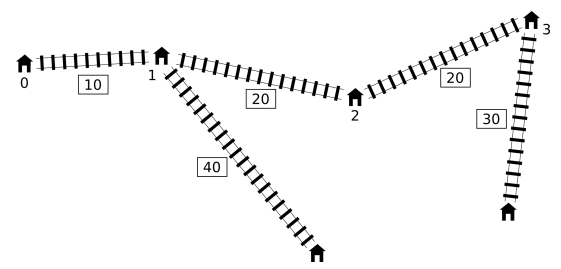
\includegraphics[scale=0.9]{1.png}

Теперь Павел хочет построить один дополнительный участок железной дороги: экспресс-линию между двумя различными (возможно соседними) станциями, расположенными \textbf{на главной линии}. Экспресс-линия будет иметь длину ровно $c$ сантиметров, независимо от того, какие две станции она будет соединять.

Каждый участок железной дороги, включая новую экспресс-линию, может быть использован в обоих направлениях. Расстоянием между двумя станциями называется минимальная длина пути, который проходит от одной станции до другой вдоль участков железной дороги. Диаметром железной дороги называется максимальное из расстояний между парами станций. Другими словами, это наименьшее число $t$, такое что расстояние между любыми двумя станциями не больше чем $t$.

Павел хочет построить экспресс-линию таким образом, чтобы итоговый диаметр был как можно меньше.

\textbf{Детали реализации}

Вы должны реализовать функцию \texttt{int64 find\_shortcut(int n, int[] l, int[] d, int c)}

\begin{itemize}
\item \texttt{n}: количество станций на главной линии,
\item \texttt{l}: расстояния между станциями на главной линии (массив длины $n - 1$),
\item \texttt{d}: длины второстепенных линий (массив длины $n$),
\item \texttt{c}: длина новой экспресс-линии.
\item Функция должна вернуть минимальный возможный диаметр железной дороги после постройки экспресс-линии.
\end{itemize}
